\documentclass[11pt,a4paper]{article}
\usepackage[margin=1in,footskip=0.5in]{geometry}
\usepackage{graphicx}
\graphicspath{{./Figures/}}

\usepackage[utf8]{inputenc}
\begin{document}
\title{Cryptocurrency Price Predictor}
\author{Benjamin Carpenter, Shuning Jin, Jacob Pauly, Tristan Larsin}
\maketitle


%%%%%%%%%%%%%%%%%%%%%%% OBJECTIVES %%%%%%%%%%%%%%%%%%%%%%%
\section{Objectives}
Our goal is to leverage machine learning to predict future prices in the cryptocurrency market. If we are successful it would empower businesses and individuals to make better financial investments. It would also assist in understanding the probabilities of risk and reward for specific investments. And the specific objectives are as follows:
\par
1) Implementing ARIMA and SVM algorithms for time series forecasting
\par
2) Using the algorithms to predict future prices based on previous prices
\par
3) Evaluating and comparing the performance of the two algorithms


%%%%%%%%%%%%%%%%%%%%%%% DATASET %%%%%%%%%%%%%%%%%%%%%%%
\section{Dataset}
Our dataset is comprised of two separate pieces.
\\ \\
The first is the historical exchanges of Bitcoin from January 1, 2012 to January 8, 2018 \cite{bitcoin_set}. The data is based on every minute update, and contains 3,161,057 observations in total. It has 8 attributes: timestamp (in Unix time), open, high, low, close, volume in BTC, volume currency, and weighted price. The csv file has a size of 212.8 MB.
\\ \\
The second is a set of 1200 top performing cryptocurrencies (sans Bitcoin) \cite{crypto_set}. The dataset includes daily records of each cryptocurrency during a time span of 1384 days from September 11, 2013 to June 26, 2017, with a total of 567,769 observations. On average, each cryptocurrency accounts for 470 records. It is characterized by 8 attributes: timestamp, opening price, daily high, daily low, closing cost, daily volume, weighted price and symbol. The csv file has a size of 36.9 MB.


%%%%%%%%%%%%%%%%%%%%%%% ALGORITHMS %%%%%%%%%%%%%%%%%%%%%%%
\section{Algorithms}
Time series forecasting is an important field in statistics. Classical models include ARIMA, GARCH, etc. In the past decade, machine learning has gained popularity in time series analyis studies, and especially Support Vector Machine (SVM) is widely applied. Currently, deep learning models stand out with their aptitude for sequential data, such as Recurrent Neural Network (RNN) and Long Short-Term Memory (LSTM).
\\ \\
In this project, we are going to use ARIMA and SVM. Below in this section, we will discuss these algorithms in details.

\subsection*{Autoregressive Integrated Moving Average Model (ARIMA)}
ARIMA model is a generalization of ARMA model, with the form:

$$\phi(B)(1-B)^dX_t=\delta+\theta(B)w_t  \qquad for ~ t = 1,2,…$$
where $\delta = \mu(1-\sum_{i=1}^{p}\phi_i)$, $w_t$ is white noise with independent and identical distributions, $\phi$ and $\theta$ are vectors of unknown fixed regression coefficients, and B is back-shifting operator defined as $B^dx_t=x_{t-d}$.

%%% 1 ARIMA %%%
\subsubsection*{(i) Model Specification}
The ARIMA$(p,d,q)$ model consists of three parts:
\par
Autoregression of order $p$: AR assumes current value $x_t$ is correlated with p past values, where p denotes the number of time lags. The autoregressive process models the trend of $x_t$.
\par
Moving average of order $q$: MA assumes current value $x_t$ is correlated with q recent white noises. The moving average smoother is to remove white noise in data and helps discover underlying long-term trend.
\par
Differencing of order $d$: time series are usually modeled by a stationary component and a nonstationary component. Performing differencing is to remove trend and produce stationarity. First difference is defined as $\nabla x_t=x_t-x_{t-1}$.

\subsubsection*{(ii) Model Fitting}
Given $p,d,q$ order for ARIMA model, we shall firstly do d-order differencing and reduce it to ARMA(p,q). Secondly, we focus on estimating parameters $\phi$ and $\theta$ in ARMA model. There are two typical techniques for such estimation: Yule-Walker estimation and maximum likehood estimation.

%%% 2 SVM %%%
\subsection*{Support Vector Machine (SVM)}

SVM constructs a hyperplane or set of hyperplanes in a high-dimensional space, which can be used for classication, regression. It allows flexible mapping of high dimensional features to capture non-linear relationships with regularization to avoid over-fitting. Our goal is draw a dividing line between classes which maximizes the the space between the line and the nearest points (known as the 'margin'). In sigma notation, we want to minimize $W(\alpha)$:

$$ W(\alpha) = \sum_{i=1}^l \alpha_i +
    \frac{1}{2} \sum_{i=1}^l \sum_{j=1}^l y_i y_j \alpha_i \alpha_j (x_i \cdot  x_j) $$

\noindent
where $\alpha$ is the vector of l non-negative Lagrange multipliers to be determined, and C is a constant. \\ \\ In order to construct $W$, Lagrange multiplication technique is applied to an optimization problems bounded by a constraint. Here, the constraint that must be satisfied is:

$$ \sum_{i=1}^l y_i \alpha_i = 0 \qquad 0 \le \alpha_i \le C \quad \forall i$$

\noindent
Note that only the closest points to the hyperplane (dividing line) are important for the problem. We could remove all other points and arrive at the same solution. Those points and their derived vectors are the 'support vectors' in SVM. By adding dimensions, we can apply SVM to many independent variables.


%%% 3 Evaluation Metrics %%%
\subsection*{Evaluation Metrics}

\subsubsection*{(i) Goodness of Fit}

\hspace{3ex}
\textbf{Akaike’s Information Criterion (AIC)}
$$AIC = log\hat{\sigma}_k^2+\frac{n+2k}{n}$$

\textbf{AIC, Bias Corrected (AICc)}
$$AICc = log\hat{\sigma}_k^2+\frac{n+k}{n-k-2}$$

\textbf{Bayesian Information Criterion (BIC)}
$$BIC = log\hat{\sigma}_k^2+\frac{klog n}{n}$$

\textbf{Mean Square Error (MSE)}
$$MSE = \frac{SSE(k)}{n-k}$$
where $\hat{\sigma}_k^2$ is the maximum likelihood estimator of variance, SSE is residual sum of squares, k is the number of parameters, and n is the number of observations.

\subsubsection*{(ii) Prediction Accuracy}

\hspace{3ex}
\textbf{Mean Absolute Percentage Error (MAPE)}
$$M = \frac{100}{n}\sum_{t=1}^{n}|\frac{A_t-F_t}{A_t}|$$
where $A_t$ is the actual value and $F_t$ is the forecast value.


%%%%%%%%%%%%%%%%%%%%%%% RELATED WORKS %%%%%%%%%%%%%%%%%%%%%%%
\section{Related Works}

\quad The work proposed by Zhang et al. \cite{zhang} is a hybrid methodology to combine the linear ARIMA and nonlinear ANN models for time series forecasting to improve performance. The empirical results with three real data sets suggest that the hybrid model outperforms its component model, and Canadian lynx data shows 19\% decrease in MSE and 8\% decrease in MAD.\\

\quad In a 2014 white paper \cite{carson}, a team from the University of Manitoba uses structural support vector machines (SSVMs) in an attempt to predict future stock market prices. SSVMs are a specialized form of supervised learning algorithm that can perform linear and non-linear regression to predict similar outcomes from past data \cite{tsochan}. In their results, they found the algorithm was performing with 78\% accuracy.\\

\quad In 2017, Facebook developed Prophet \cite{taylor}, which is a powerful tool for time series forecasting available in Python and R. Prophet is aimed at efficiently producing high quality forecasts with large number of time series data points. They used the generalized additive model (GAM), which is based on time series decomposition. Three main components are used: trend, seasonality, and holiday. GAM has great flexibility when used non-parametrically.\\

\quad Autoregressive Integrated Moving Average (ARIMA) was used by Vinay et al. \cite{vinay} to predict road-traffic volume. ARIMA is used for short-term and long-term historical data. There are several variations of ARIMA that are best suited for given problems. This research tested all of the variations to compare the different accuracies of his road-traffic volume predictions. Some variations have more overhead than others, but lack accuracy. Based purely on accuracy ARIMA-GARCH outperformed all other variations of ARIMA.\\

\quad In a 2016 paper \cite{ved}, a team used a support vector machine (SVM) and kernel functions to forecast the stock market. They separated the stock market changes into two classifications, rising and declining. When rising, the value at $x-1$ is less than that at $x$. When declining, the value at $x+1$ is less than that at $x$. The types of SVM kernels used were linear, polynomial, and radial basis. The most accurate SVM kernel performed with an 88.34\% accuracy.\\

\quad Additional methods used by David Sheehan \cite{sheehan} including the long short term memory (LSTM) model, which is a type of deep learning that can predict cryptocurrency prices. LSTM models are well suited for time series data because loops in neural nets allow for persistent data. In essence, they can remember how time series data has behaved in the past. Sheehan decided to use the same Bitcoin dataset that we have chosen. This dataset includes Bitcoin’s details at a one-minute interval from January 2012 through January 2018. This provided him with six years of data. Testing his algorithm from July 1st, 2017 through November 1st, 2017 he received a mean absolute error (MAE) of 0.0392. \\

\quad In our project, we will apply SVM and ARIMA for cryptocurrency price prediction. While SVM and ARIMA have been widely applied for stock price forecasting, we want to investigate their predictive power in the context of cryptocurrency. Also, we are interested in comparing the performance of the these two algorithms.

%%%%%%%%%%%%%%%%%%%%%%% TIME TABLE %%%%%%%%%%%%%%%%%%%%%%%
\section{Time Table}
\begin{tabular}{ | p{1cm} | p{3cm} | p{4.5cm} | p{3cm} | p{2cm} | }
  \hline
  Date & Action & Notes & Deliverables & Status\\ \hline
  2.1 & Written Project Proposal & Write out the description of our project, algorithms and previous works. & Project Proposal & Completed\\ \hline
  2.6 & Preprocessing & Deal with missing values (depends on models), data transformation. & Prepared dataset & Completed\\ \hline
  2.12 & Structure project \& start development & Layout the structure of our project (file wise). Delegate roles for each section of our project. Start working on respective sections. Preliminary data analysis. & File structure and data set uploaded to Git repository.& Completed\\ \hline
  2.25 & Implement ARIMA algorithm & Testable algorithm. & Testable project& Partially done\\ \hline
  3.20 & Implement SVM algorithm & Both algorithms are now implemented and ready to be tested & 2 testable algorithms & Partially done\\ \hline
  4.1 & Run ARIMA on bitcoin dataset & Run algorithms to access final accuracies.  & Accuracy of algorithms   &  Completed \\ \hline
  4.12 & Run SVM on bitcoin dataset & Run algorithms to access final accuracies.  & Accuracy of algorithms &  Not started \\ \hline
  4.15 & Compare the two algorithms & Compare their train errors and test errors.  & Analysis of algorithms &  Not started \\ \hline
  4.24 & Complete project & Submit final report & Final algorithms and accuracy & Not started\\ \hline
\end{tabular}
\\


% \subsection*{Justification}
% A previous version of this proposal had an unreasonable completion date for the time series algorithms, including finishing initial implementation before they had been introduced in the course.

%%%%%%%%%%%%%%%%%%%%%%%%%%
\subsection*{Progress}
Since Project Progress Report 1, we start with SVM implementation and continue with ARIMA implementation.
\\ \\
For ARIMA model, we carry out a comprehensive data analysis of the bitcoin historical dataset in R.

\subsubsection*{(i) Preprocessing}
The original dataset is based on every minute data from 2012-01-01 to 2018-01-08. Initially, we transform it to daily data by adopting the observations on 00:00 for each day. We use the close price as both the response variable and the explanatory variable. The plot shows the trend in early years is relatively trivial. Thus, we decide to only use data from 2017-01-01 to 2018-01-01, which has 366 observations. To stablize the variance, log transform is applied.

%% plot for 2012-2018, 2017-2018 log tranform

\begin{center}
   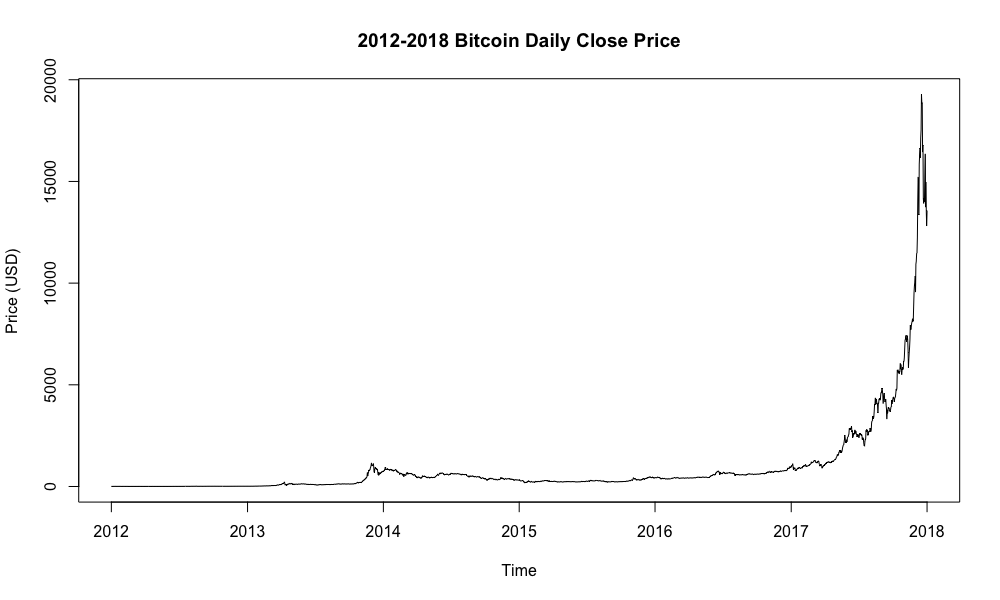
\includegraphics[width=0.8\textwidth]{2012-2018.png}
\end{center}
\graphicspath{{./Figures/}}

\begin{center}
   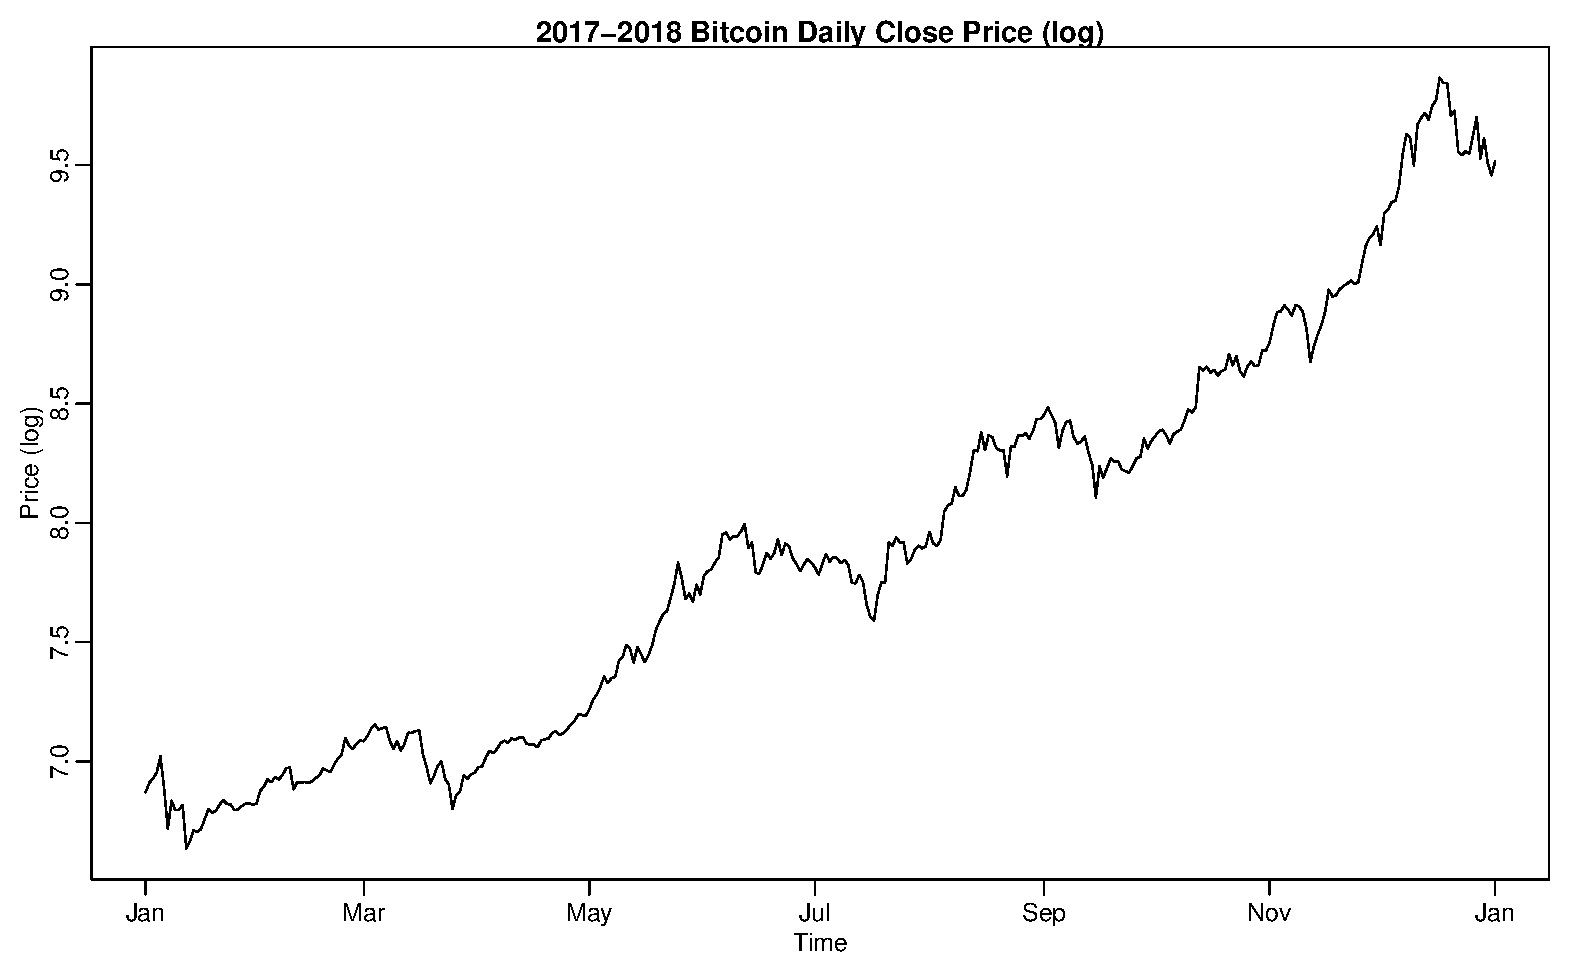
\includegraphics[width=0.8\textwidth]{2017-2018_log.eps}
\end{center}
\graphicspath{{./Figures/}}


\subsubsection*{(ii) Hyperparameter}
There are three hyperparameters in ARIMA(p,d,q) model. \\
We want to identify the differencing order d, and sample ACF $\hat\rho(h)$ serves a criterion - that is, slow decay in ACF indicates a need for differencing. Since the ACF of our data shows such pattern, we do first differencing. After that, the ACF suffices and no futher differencing is needed. Hence, we decide d=1. $\nabla log(x_t)$ is also called the return or growth rate. \\


%% ACF1, first differenced data
\begin{center}
   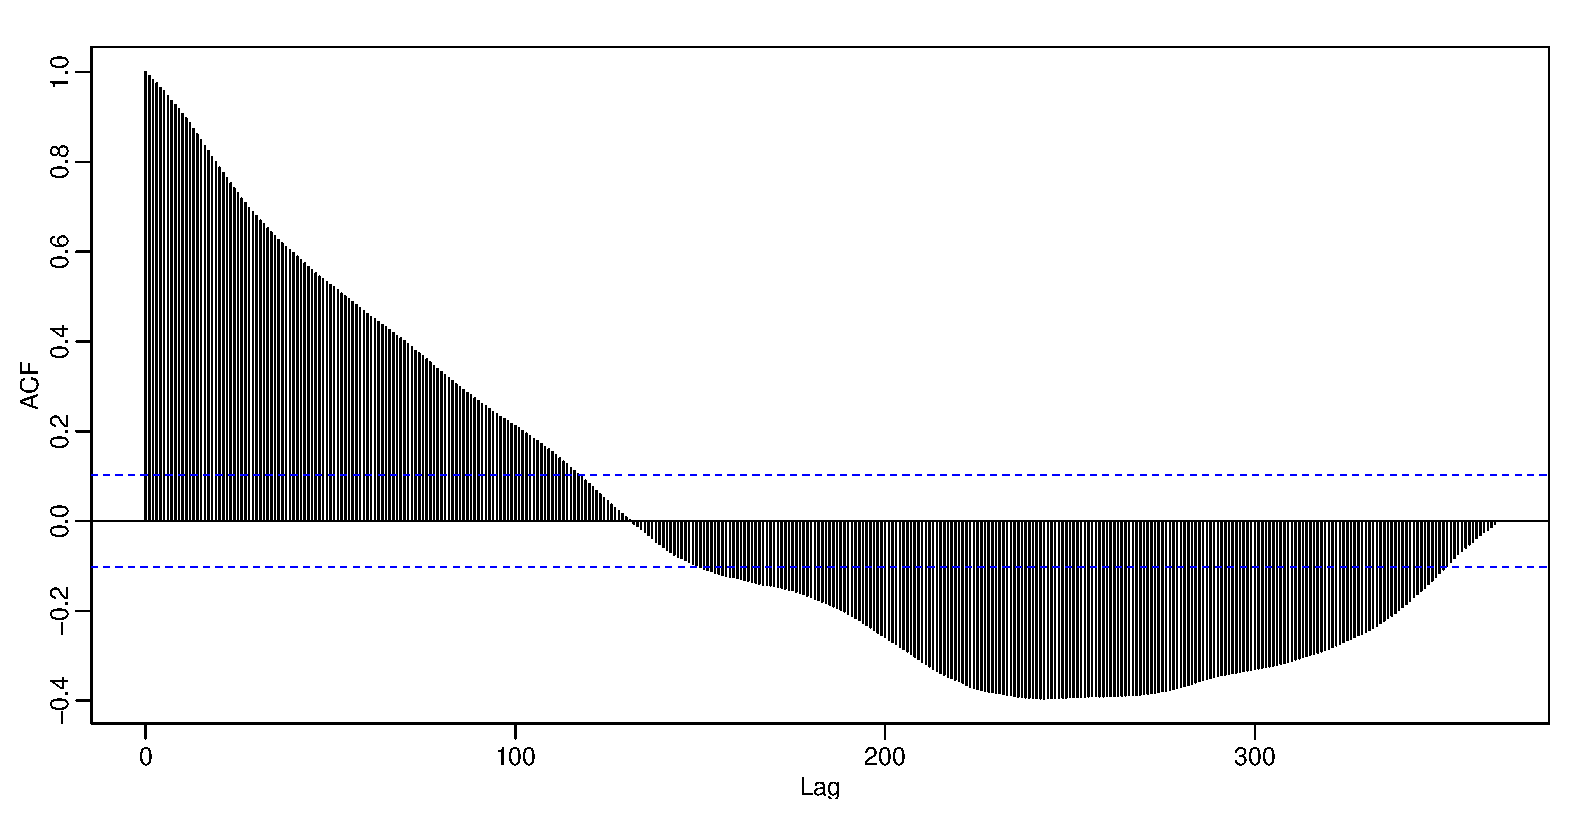
\includegraphics[width=0.8\textwidth]{acf1.eps}
\end{center}
\graphicspath{{./Figures/}}

\begin{center}
   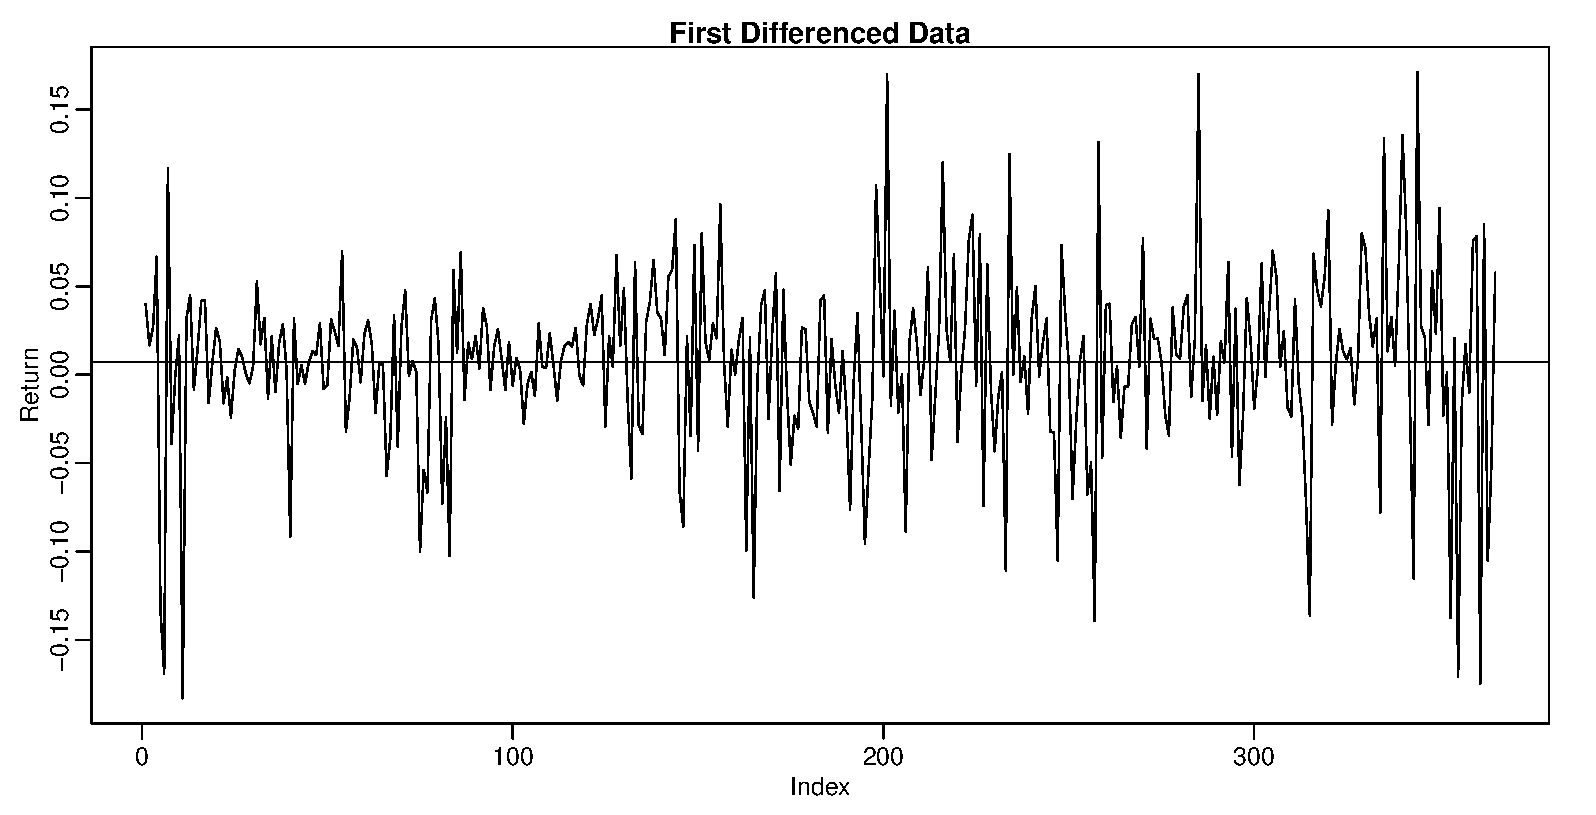
\includegraphics[width=0.8\textwidth]{return.eps}
\end{center}
\graphicspath{{./Figures/}}

We also need to identify the autoregressive order p and movering average order q. Above all, we need to determine if p=0 or q=0, which correspond to MA(q) or AR(p) respectively. We use the sample ACF and PACF behavior as a guide. Since there are no cut off after certain lags and both ACF and PACF tail off, we can conclude p and q are nonzero, leading to ARMA(p,q) model. For simplicity, we assign p=1 and q=1. That is, we adopt ARMA(p=1,q=1) for the first differenced data, which corresponds to ARIMA(p=1,d=1,q=1) for the original log transformed data. The model adequency will be more rigorously examined below.

%%  ACF2, PACF2
\begin{center}
   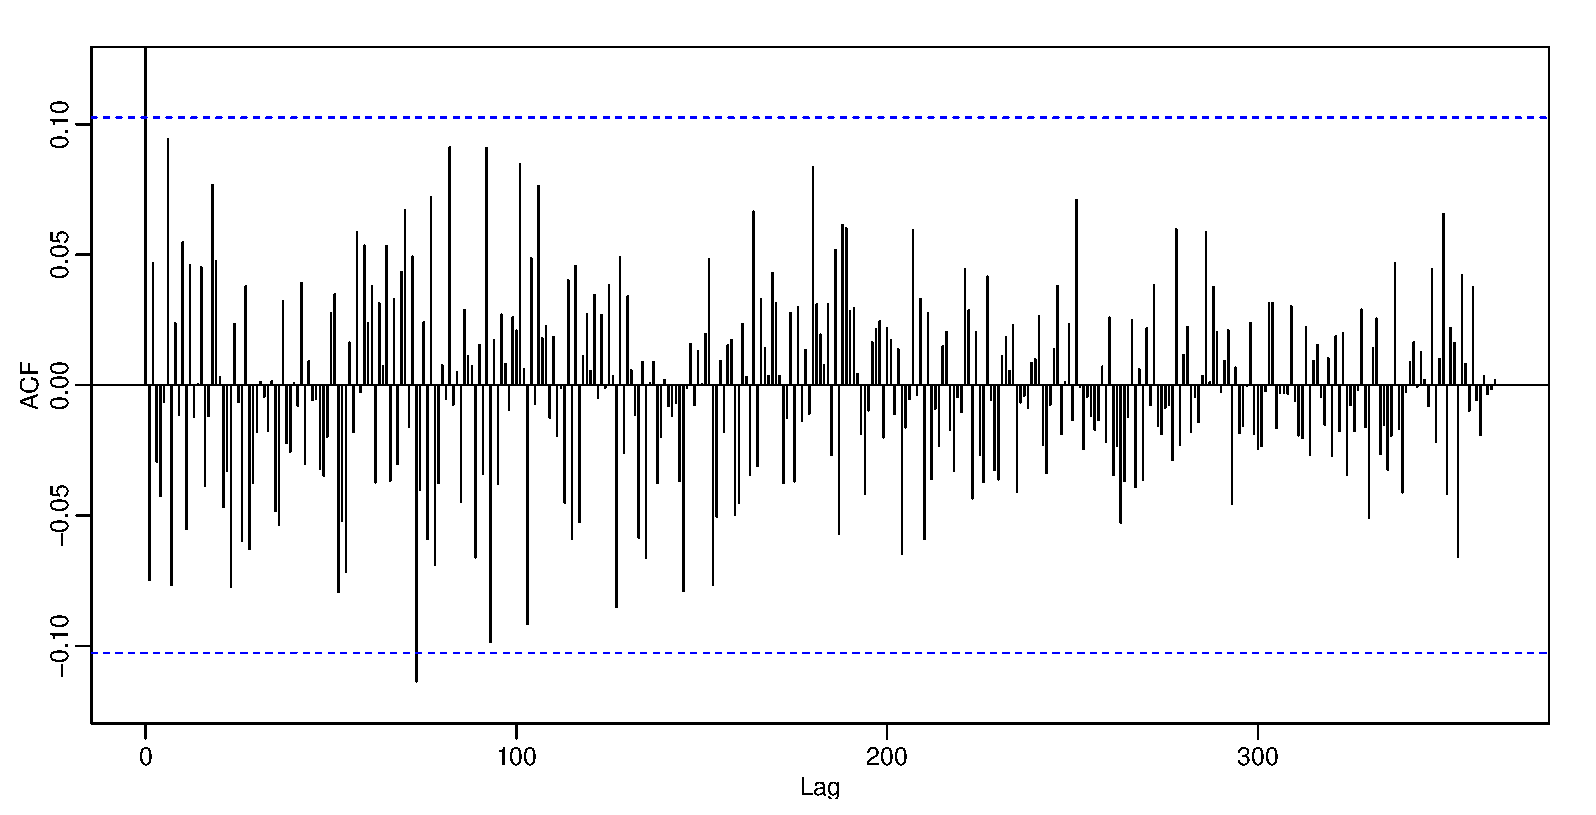
\includegraphics[width=0.8\textwidth]{acf2.eps}
\end{center}
\graphicspath{{./Figures/}}

\begin{center}
   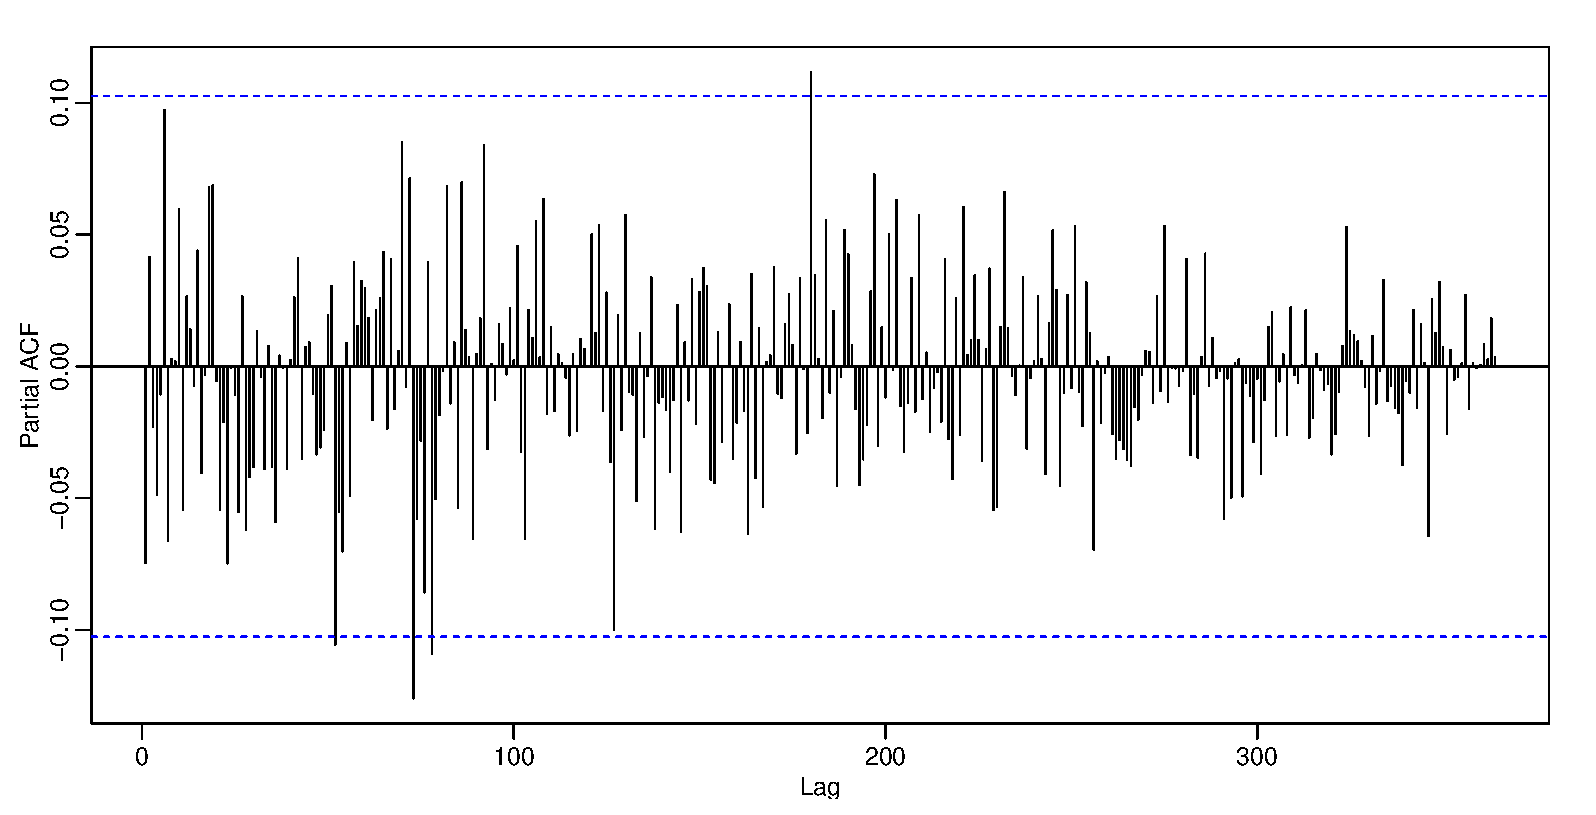
\includegraphics[width=0.8\textwidth]{pacf2.eps}
\end{center}
\graphicspath{{./Figures/}}

\subsubsection*{(iii) Model Checking}
With all three hyperparameters specified, we carry out preliminary model checking by residual analysis. Applying the data, the 'sarima' method in 'astsa' package gives 4 diagnostic plots of standardized residuals

$$ e_t = \frac{x_t - \hat{x}_{t}^{t-1}} {\sqrt{\hat{P}_{t}^{t-1}}} $$
where $\hat{x}_{t}^{t-1}$ is the one-step-ahead prediction of $x_t$,
and $\hat{P}_{t}^{t-1}$ is the estimated one-step-ahead error variance. \\

\par
(a) Ideally, the residuals should have iid distribution with $\mu=0$ and $\sigma^2=1$. The time plot shows no obvious patterns and the mean is around 0. But a few values exceed 3 standard deviations in magnitude, which could be outliers.
\par
(b) To check the assumption of randomness, we inspect the sample ACF. There are no significantly large values, indicating no apparent departure from this assumption.
\par
(c) The normal Q-Q plot is heavy tailed. This means the assumption of normality may not strictly hold.
\par
(d) The p values for Ljung-Box Q-statistic are large (greater than 0.2), thus we do not reject the null hypothesis of model adequency.
\\ \\ Thus, we conclude that this model is suitable for our dataset in general.

%% residual analysis
\begin{center}
   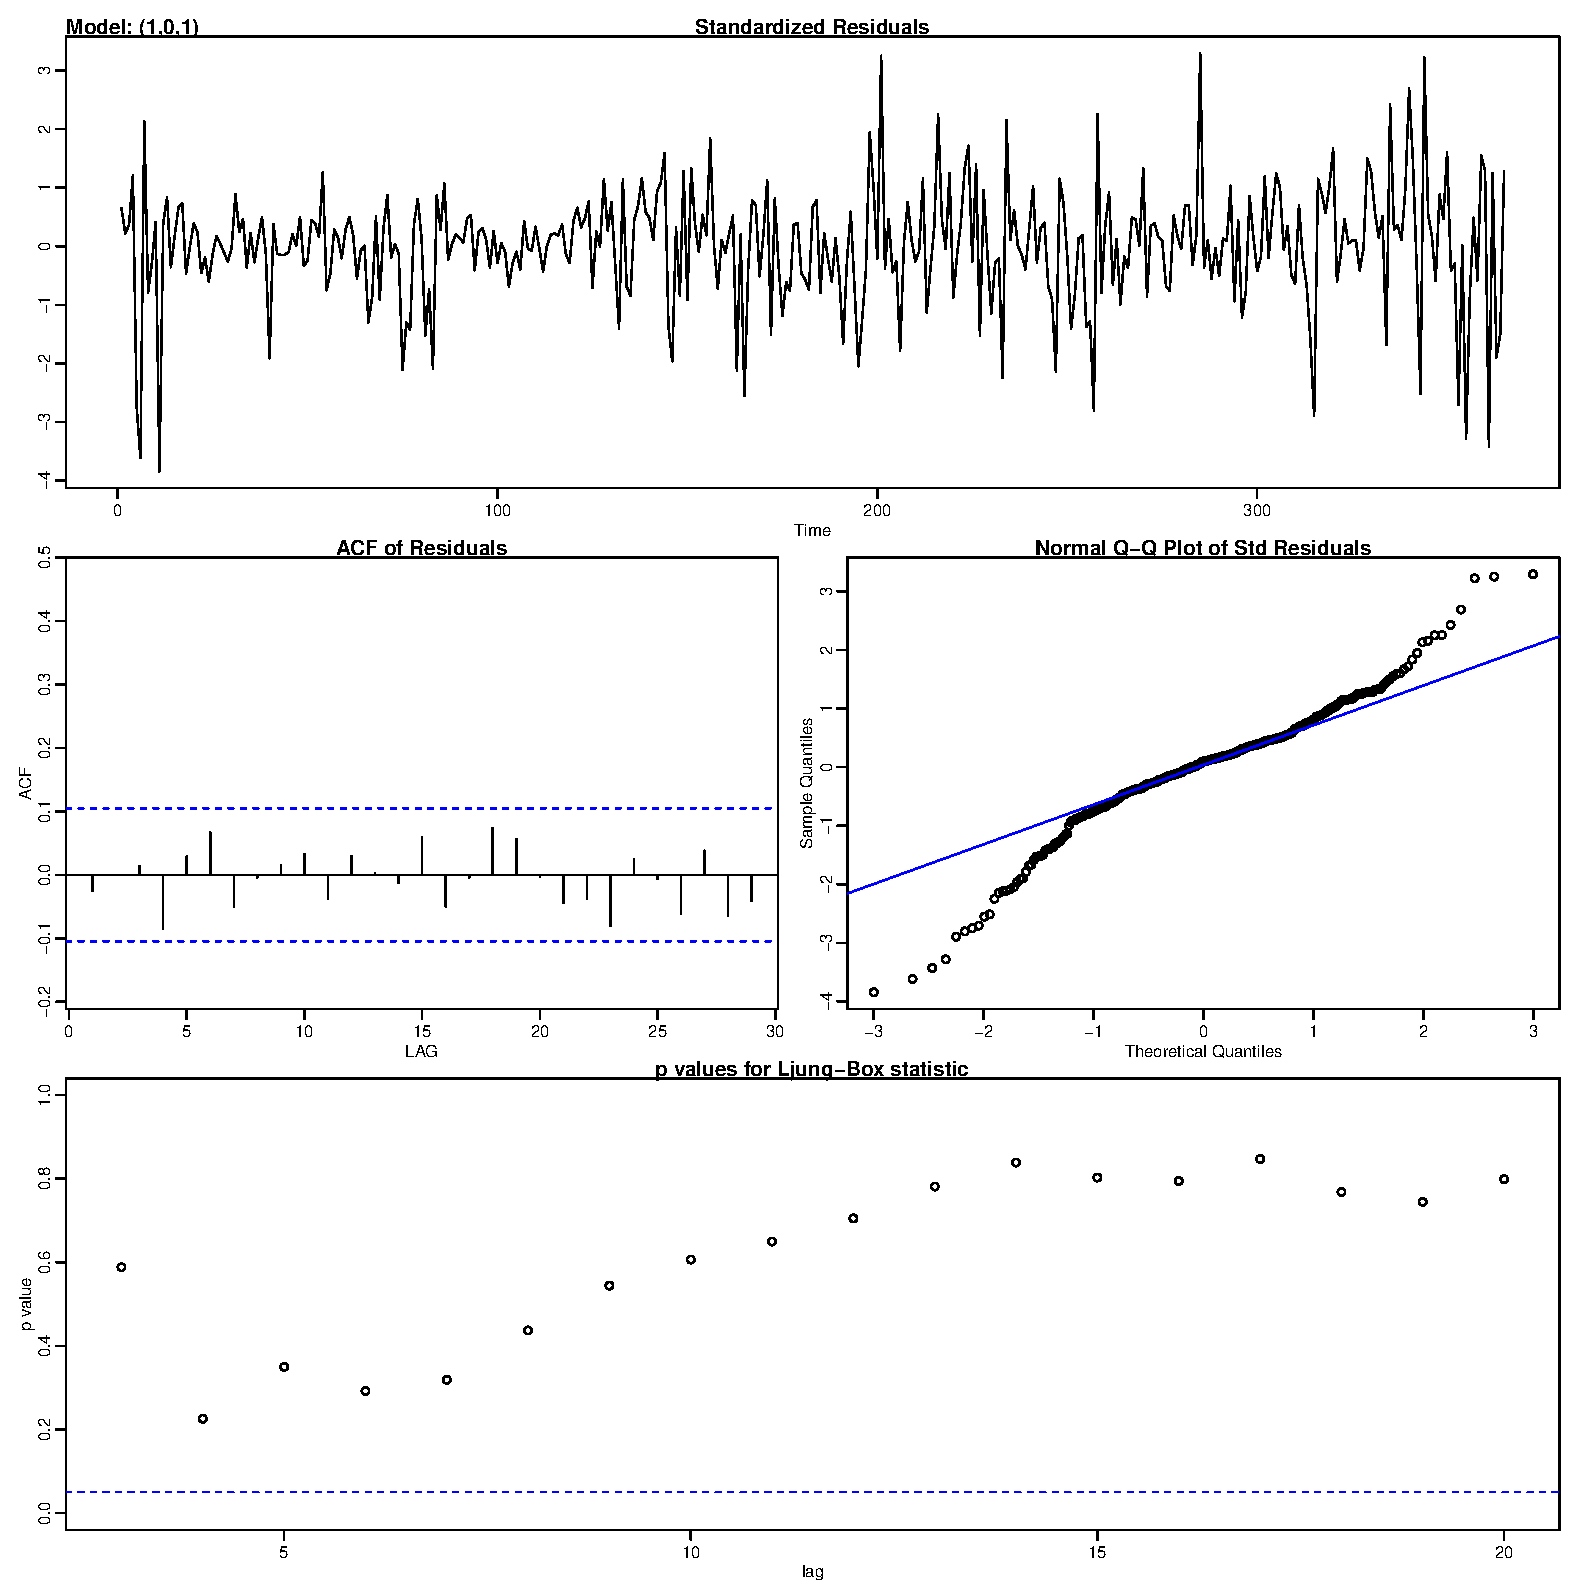
\includegraphics[width=0.8\textwidth]{diagnosis.eps}
\end{center}
\graphicspath{{./Figures/}}


\subsubsection*{(iv) Model Performance}

First, we divide the data into training set and testing set using a 90:10 split. Due to the nature of time series data, we could not do random sampling here. Since 1 data point is lost due to previous differencing, we have 365 data in total, with the first 328 for train and the last 37 for test. Second, we fit the model with training data. The train error is measured by MSE = 0.002159. Third, we make m-step-ahead long range forecast based on historical (train) data, with m = test size = 37. By comparing predicted values with test data, we derive test error in two ways. The test MSE is 0.006412. And MAPE is 23.40647.

%% prediction

\subsection*{Remaining Work}
1. For ARIMA model, we have accomplished 2 main components: differencing and autoregression. We still need to incorporate the moving average component.  \\
2. For SVM model, we need to finish its implementation. \\
3. We have finished data analysis using ARIMA. And we need to do data analysis using SVM. The method will be similar to the former. \\
\\ The work will be done within next two or three weeks.



\clearpage

%%%%%%%%%%%%%%%%%%%%%%% REFERENCES %%%%%%%%%%%%%%%%%%%%%%%

\begin{thebibliography}{10}

    \bibitem{bitcoin_set} 
        \textit{https://www.kaggle.com/mczielinski/bitcoin-historical-data}
    \bibitem{crypto_set}
        \textit{https://www.kaggle.com/akababa/cryptocurrencies}
    \bibitem{carson}
        \textit{Carson Kai-Sang Leung, Richard Kyle MacKinnon, and Yang Wang.
                A machine learning approach for stock price prediction. In
                Proceedings of the 18th International Database Engineering \&
                Applications Symposium (IDEAS '14), Ana Maria Almeida, Jorge
                Bernardino, and Elsa Ferreira Gomes (Eds.).
                ACM, New York, NY, USA, 274-277. 2014.\\
                DOI: https://doi.org/10.1145/2628194.2628211}
    \bibitem{sheehan}
        \textit{David Sheehan. Predicting Cryptocurrency Prices With
                Deep Learning. (November 2017). 2017.}
    \bibitem{shumway}
         \textit{Shumway RH, Stoffer DS. Time Series Analysis and Its Applications. New York: Springer. 2000.}
    \bibitem{taylor}
        \textit{Taylor SJ, Letham B. Forecasting at scale. PeerJ
                Preprints 5:e3190v2 2017.\\ DOI: https://doi.org/10.7287/peerj.preprints.3190v2}
    \bibitem{tsochan}
        \textit{Tsochantaridis, Ioannis, et al. Support Vector Machine
                Learning for Interdependent and Structured Output Spaces.
                Twenty-First International Conference on Machine Learning -
                ICML '04, 2004.\\
                DOI:10.1145/1015330.1015341.}
    \bibitem{ved}
        \textit{Ved Prakash Upadhyay, Subhash Panwar, Ramchander Merugu, and
                Ravindra Panchariya. Forecasting Stock Market Movements Using Various
                Kernel Functions in Support Vector Machine. In Proceedings of the
                International Conference on Advances in Information Communication
                Technology \& Computing (AICTC '16), S. K. Bishnoi, Manoj Kuri, and
                Vishal Goar (Eds.). ACM, New York, NY, USA, Article 107 , 5 pages. 2016.\\
                DOI: https://doi.org/10.1145/2979779.2979886}
    \bibitem{vinay}
         \textit{Vinay B. Gavirangaswamy, Gagan Gupta, Ajay Gupta, and Rajeev
                Agrawal. Assessment of ARIMA-based prediction techniques for
                road-traffic volume. In Proceedings of the Fifth International
                Conference on Management of Emergent Digital EcoSystems (MEDES '13).
                ACM, New York, NY, USA, 246-251. 2013.\\
                DOI: http://dx.doi.org/10.1145/2536146.2536176}
    \bibitem{zhang}
        \textit{Zhang GP. Times series forecasting using a hybrid ARIMA and
                neural network model. Neurocomputing 50:159–75 2003.}

    \end{thebibliography}
\end{document}

